\documentclass[12pt,afrikaans, english,letterpaper,oneside,
openany]{memoir}

%==== Graphics and Color ============================================
\usepackage{graphicx}%........................... Graphicx loaded in usthesis
\usepackage{color}%.............................. Color setup
\usepackage{eso-pic}%............................ Shipout commands for watermark
    \newcommand*{\WaterMark}[2][0.15\paperwidth]{%
        \AddToShipoutPicture*{\AtTextCenter{%
                \parbox[t]{0pt}{\makebox[0pt][c]{%
                    \includegraphics[width=#1]{#2}}}}}}

\usepackage[masters-t, goldenblock,]{usthesis} % option to replace masters-t with PhD 
\usepackage{lmodern}
\usepackage{amssymb,amsmath}
\usepackage{ifxetex,ifluatex}
\usepackage{textcomp}
\usepackage{bm}
\usepackage{fixltx2e} % provides \textsubscript
\ifnum 0\ifxetex 1\fi\ifluatex 1\fi=0 % if pdftex
  \usepackage[T1]{fontenc}
  \usepackage[utf8]{inputenc}
\else % if luatex or xelatex
  \usepackage{unicode-math}
  \defaultfontfeatures{Ligatures=TeX,Scale=MatchLowercase}
\fi
% use upquote if available, for straight quotes in verbatim environments
\IfFileExists{upquote.sty}{\usepackage{upquote}}{}
% use microtype if available
\IfFileExists{microtype.sty}{%
\usepackage[]{microtype}
\UseMicrotypeSet[protrusion]{basicmath} % disable protrusion for tt fonts
}{}
\PassOptionsToPackage{hyphens}{url} % url is loaded by hyperref
\usepackage[unicode=true]{hyperref}
\usepackage[capitalize]{cleveref} % delete if not working
\hypersetup{
            pdftitle={The relationship between illicit cigarettes and the legal tobacco market in South Africa},
            pdfauthor={Cassandra Pengelly},
            pdfborder={0 0 0},
            breaklinks=true}
\urlstyle{same}  % don't use monospace font for urls
\ifnum 0\ifxetex 1\fi\ifluatex 1\fi=0 % if pdftex
  \usepackage[shorthands=off,main=]{babel}
\else
  \usepackage{polyglossia}
  \setmainlanguage[]{}
\fi
\usepackage{usnomencl}
\usepackage{acronym}
%\usepackage{natbib}
%\bibliographystyle{plainnat}
\usepackage{usbib}%.............................. Bibliography    (in usthesis pack)
    \bibliographystyle{usmeg-a}
    \renewcommand\bibfont{\small}

    %% For usmeg-a, the bib is a list of references. If you
    %% are using usmeg-n comment out the following lines
    \addto{\captionsafrikaans}{\renewcommand{\bibname}{Lys van Verwysings}}
    \addto{\captionsenglish}{\renewcommand{\bibname}{List of References}}
\IfFileExists{parskip.sty}{%
\usepackage{parskip}
}{% else
\setlength{\parindent}{0pt}
\setlength{\parskip}{6pt plus 2pt minus 1pt}
}
\setlength{\emergencystretch}{3em}  % prevent overfull lines
\providecommand{\tightlist}{%
  \setlength{\itemsep}{0pt}\setlength{\parskip}{0pt}}
\setcounter{secnumdepth}{5}
% Redefines (sub)paragraphs to behave more like sections
\ifx\paragraph\undefined\else
\let\oldparagraph\paragraph
\renewcommand{\paragraph}[1]{\oldparagraph{#1}\mbox{}}
\fi
\ifx\subparagraph\undefined\else
\let\oldsubparagraph\subparagraph
\renewcommand{\subparagraph}[1]{\oldsubparagraph{#1}\mbox{}}
\fi

% set default figure placement to htbp
\makeatletter
\def\fps@figure{htbp}
\makeatother

\usepackage{subfig}
\usepackage{array}
\usepackage{caption}
\usepackage{graphicx}
\usepackage{siunitx}
\usepackage[normalem]{ulem}
\usepackage{colortbl}
\usepackage{multirow}
\usepackage{hhline}
\usepackage{calc}
\usepackage{tabularx}
\usepackage{threeparttable}
\usepackage{wrapfig}
\usepackage{adjustbox}
\usepackage{hyperref}

\title{\bfseries\AorE{Hierdie is die titel van my
tesis\\[1ex]\normalfont\small\itshape(``The relationship between illicit
cigarettes and the legal tobacco market in South Africa'')}{The
relationship between illicit cigarettes and the legal tobacco market in
South Africa}}
\providecommand{\subtitle}[1]{}
\subtitle{An econometric analysis}
%\author{Cassandra Pengelly}
\author{C.~Pengelly}{Cassandra Pengelly}
\address{\AorE{%-- Afrikaans ----------------------------------------
        Departement van Ekonomie,\\
        Universiteit van Stellenbosch,\\
        Privaatsak X1, Matieland 7602, Suid Afrika.%
             }{%-- English ------------------------------------------
        Department of Economics,\\
        University of Stellenbosch,\\
        Private Bag X1, Matieland 7602, South Africa.
             }}
% \date{}
\degree{\AorE{MCom (Ekonomie)}{MCom (Economics)}}
       {\AorE{Magister in Ekonomie}
             {Master in Economics}}
\faculty{\AorE{Fakulteit Ekonomiese en Bestuurswetenskappe}
              {Faculty of Economic and Management Sciences}}

\supervisor{Prof.~W.~H. Boshoff}
%\cosupervisor{$}

\setdate{4}{2023}

% \SetSponsor{The financial assistance of the Graduate School of Economic and Management Sciences (GEM) towards this research is hereby acknowledged. Opinions expressed are those of the author and are not to be attributed to GEM.}

%\maxsecnumdepth{subsubsection}
%\maxtocdepth{section}

%\renewcommand{\baselinestretch}{1.5}
%\onehalfspacing
\linespread{1.213}

\begin{document}
 \frontmatter
  \WaterMark{./images/sun_logo.png}
  \TitlePage
 
\DeclarationPage

\input{abstract.Rmd}

\input{acknowledgements.Rmd}
\clearpage

{
\setcounter{tocdepth}{2}
\tableofcontents
\clearpage
}
\setcounter{lofdepth}{2}
\listoffigures
\clearpage
\listoftables
\clearpage



\mainmatter
   \setsecnumdepth{subsubsection}
   \numberwithin{equation}{section}
   \numberwithin{figure}{chapter}
   \numberwithin{table}{chapter}
\hypertarget{introduction}{%
\chapter{Introduction}\label{introduction}}

This study examines the relationship between the legal and illegal
tobacco markets in South Africa. Section \ref{data} discusses the data
used and how it was cleaned. Section \ref{methodology} explains the
methodology, where a VECM model is presented. The final section details
discussion points (\ref{analysis}). The appendix contains the full model
outputs.

\hypertarget{the-tobacco-industry-in-south-arica}{%
\chapter{The tobacco industry in South
Arica}\label{the-tobacco-industry-in-south-arica}}

The concern around the illict tobacco market twofold. Firstly, access to
cheaper cigarettes

\hypertarget{data}{%
\chapter{\texorpdfstring{Data \label{data}}{Data }}\label{data}}

The sample period for this study runs from January 2012 to March 2020.
Monthly data is used such that there are 99 observation points for each
variable in the data set. One of the advantages of using monthly data
rather than annual data is that it allows for more degrees of freedom.
The data used includes figures for the prices and volumes of cigarettes
in South Africa, tobacco excise duties, VAT, and disposable income. To
prepare the data for analysis the most popular price category (MPPC) was
identified as the 20-cigarette pack. Then a weighted average of
before-tax 20-pack prices was used as a base price. The excise duty per
20's pack and VAT and were then added to the base price to calculate the
price of licit cigarettes. The licit, illicit and disposable income
amounts were adjusted for inflation, taking December 2016 as the base
month and year. All of the variables have been transformed into log
form.

\begin{center}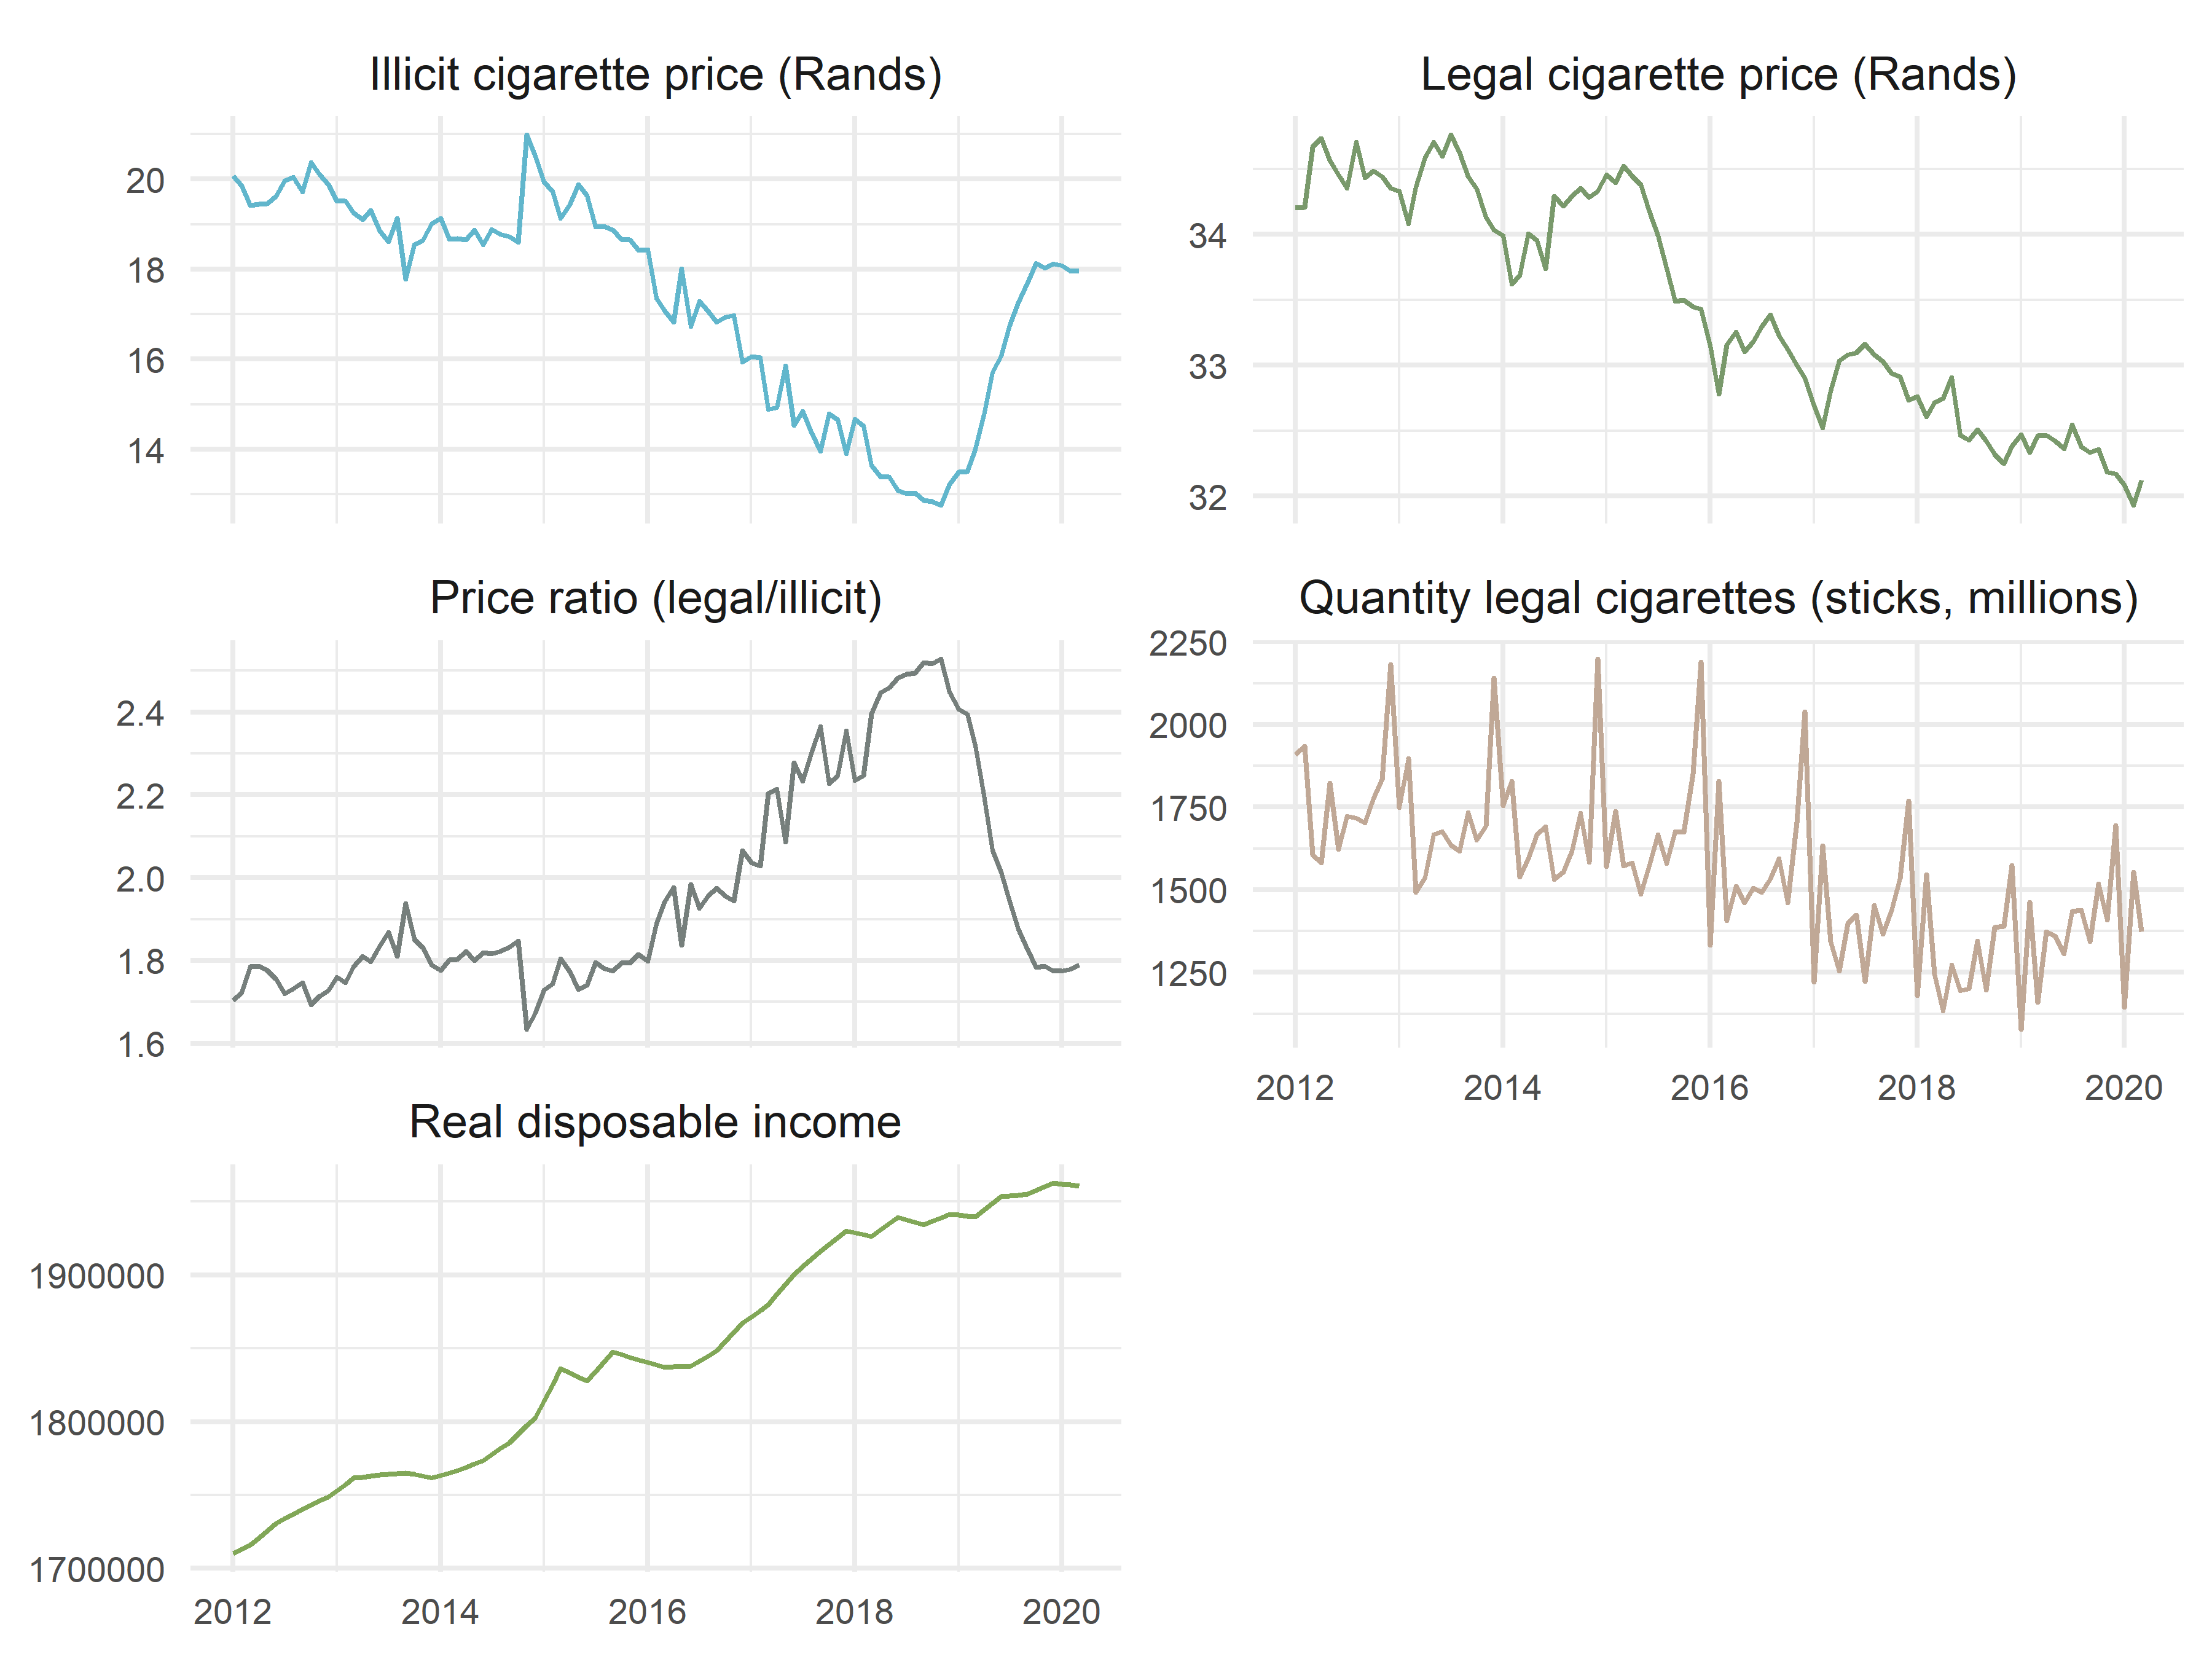
\includegraphics{index_files/figure-latex/graphs-1} \end{center}

\hypertarget{methodology}{%
\chapter{\texorpdfstring{Methodology
\label{methodology}}{Methodology }}\label{methodology}}

\hypertarget{stationarity}{%
\section{\texorpdfstring{Stationarity
\label{stationarity}}{Stationarity }}\label{stationarity}}

Running the ADF tests.

 
  \providecommand{\huxb}[2]{\arrayrulecolor[RGB]{#1}\global\arrayrulewidth=#2pt}
  \providecommand{\huxvb}[2]{\color[RGB]{#1}\vrule width #2pt}
  \providecommand{\huxtpad}[1]{\rule{0pt}{#1}}
  \providecommand{\huxbpad}[1]{\rule[-#1]{0pt}{#1}}

\begin{table}[ht]
\begin{centerbox}
\begin{threeparttable}
\captionsetup{justification=centering,singlelinecheck=off}
\caption{This is my caption \label{tab:adf}}
 \label{tab:stationarityResults}
\setlength{\tabcolsep}{0pt}
\begin{tabular}{l l l l l}


\hhline{>{\huxb{0, 0, 0}{0.4}}->{\huxb{0, 0, 0}{0.4}}->{\huxb{0, 0, 0}{0.4}}->{\huxb{0, 0, 0}{0.4}}->{\huxb{0, 0, 0}{0.4}}-}
\arrayrulecolor{black}

\multicolumn{1}{!{\huxvb{0, 0, 0}{0}}r!{\huxvb{0, 0, 0}{0}}}{\huxtpad{2pt + 1em}\raggedleft \hspace{2pt} \textbf{{\fontsize{10pt}{12pt}\selectfont Statistic}} \hspace{2pt}\huxbpad{2pt}} &
\multicolumn{1}{r!{\huxvb{0, 0, 0}{0}}}{\huxtpad{2pt + 1em}\raggedleft \hspace{2pt} \textbf{{\fontsize{10pt}{12pt}\selectfont p.value}} \hspace{2pt}\huxbpad{2pt}} &
\multicolumn{1}{r!{\huxvb{0, 0, 0}{0}}}{\huxtpad{2pt + 1em}\raggedleft \hspace{2pt} \textbf{{\fontsize{10pt}{12pt}\selectfont parameter}} \hspace{2pt}\huxbpad{2pt}} &
\multicolumn{1}{l!{\huxvb{0, 0, 0}{0}}}{\huxtpad{2pt + 1em}\raggedright \hspace{2pt} \textbf{{\fontsize{10pt}{12pt}\selectfont method}} \hspace{2pt}\huxbpad{2pt}} &
\multicolumn{1}{l!{\huxvb{0, 0, 0}{0}}}{\huxtpad{2pt + 1em}\raggedright \hspace{2pt} \textbf{{\fontsize{10pt}{12pt}\selectfont alternative}} \hspace{2pt}\huxbpad{2pt}} \tabularnewline[-0.5pt]


\hhline{>{\huxb{0, 0, 0}{0.4}}->{\huxb{0, 0, 0}{0.4}}->{\huxb{0, 0, 0}{0.4}}->{\huxb{0, 0, 0}{0.4}}->{\huxb{0, 0, 0}{0.4}}-}
\arrayrulecolor{black}

\multicolumn{1}{!{\huxvb{0, 0, 0}{0}}r!{\huxvb{0, 0, 0}{0}}}{\huxtpad{2pt + 1em}\raggedleft \hspace{2pt} {\fontsize{10pt}{12pt}\selectfont -4.67} \hspace{2pt}\huxbpad{2pt}} &
\multicolumn{1}{r!{\huxvb{0, 0, 0}{0}}}{\huxtpad{2pt + 1em}\raggedleft \hspace{2pt} {\fontsize{10pt}{12pt}\selectfont 0.0100} \hspace{2pt}\huxbpad{2pt}} &
\multicolumn{1}{r!{\huxvb{0, 0, 0}{0}}}{\huxtpad{2pt + 1em}\raggedleft \hspace{2pt} {\fontsize{10pt}{12pt}\selectfont 4} \hspace{2pt}\huxbpad{2pt}} &
\multicolumn{1}{l!{\huxvb{0, 0, 0}{0}}}{\huxtpad{2pt + 1em}\raggedright \hspace{2pt} {\fontsize{10pt}{12pt}\selectfont Augmented Dickey-Fuller Test} \hspace{2pt}\huxbpad{2pt}} &
\multicolumn{1}{l!{\huxvb{0, 0, 0}{0}}}{\huxtpad{2pt + 1em}\raggedright \hspace{2pt} {\fontsize{10pt}{12pt}\selectfont stationary} \hspace{2pt}\huxbpad{2pt}} \tabularnewline[-0.5pt]


\hhline{}
\arrayrulecolor{black}

\multicolumn{1}{!{\huxvb{0, 0, 0}{0}}r!{\huxvb{0, 0, 0}{0}}}{\huxtpad{2pt + 1em}\raggedleft \hspace{2pt} {\fontsize{10pt}{12pt}\selectfont -1.44} \hspace{2pt}\huxbpad{2pt}} &
\multicolumn{1}{r!{\huxvb{0, 0, 0}{0}}}{\huxtpad{2pt + 1em}\raggedleft \hspace{2pt} {\fontsize{10pt}{12pt}\selectfont 0.8084} \hspace{2pt}\huxbpad{2pt}} &
\multicolumn{1}{r!{\huxvb{0, 0, 0}{0}}}{\huxtpad{2pt + 1em}\raggedleft \hspace{2pt} {\fontsize{10pt}{12pt}\selectfont 4} \hspace{2pt}\huxbpad{2pt}} &
\multicolumn{1}{l!{\huxvb{0, 0, 0}{0}}}{\huxtpad{2pt + 1em}\raggedright \hspace{2pt} {\fontsize{10pt}{12pt}\selectfont Augmented Dickey-Fuller Test} \hspace{2pt}\huxbpad{2pt}} &
\multicolumn{1}{l!{\huxvb{0, 0, 0}{0}}}{\huxtpad{2pt + 1em}\raggedright \hspace{2pt} {\fontsize{10pt}{12pt}\selectfont stationary} \hspace{2pt}\huxbpad{2pt}} \tabularnewline[-0.5pt]


\hhline{}
\arrayrulecolor{black}

\multicolumn{1}{!{\huxvb{0, 0, 0}{0}}r!{\huxvb{0, 0, 0}{0}}}{\huxtpad{2pt + 1em}\raggedleft \hspace{2pt} {\fontsize{10pt}{12pt}\selectfont -3.31} \hspace{2pt}\huxbpad{2pt}} &
\multicolumn{1}{r!{\huxvb{0, 0, 0}{0}}}{\huxtpad{2pt + 1em}\raggedleft \hspace{2pt} {\fontsize{10pt}{12pt}\selectfont 0.0739} \hspace{2pt}\huxbpad{2pt}} &
\multicolumn{1}{r!{\huxvb{0, 0, 0}{0}}}{\huxtpad{2pt + 1em}\raggedleft \hspace{2pt} {\fontsize{10pt}{12pt}\selectfont 4} \hspace{2pt}\huxbpad{2pt}} &
\multicolumn{1}{l!{\huxvb{0, 0, 0}{0}}}{\huxtpad{2pt + 1em}\raggedright \hspace{2pt} {\fontsize{10pt}{12pt}\selectfont Augmented Dickey-Fuller Test} \hspace{2pt}\huxbpad{2pt}} &
\multicolumn{1}{l!{\huxvb{0, 0, 0}{0}}}{\huxtpad{2pt + 1em}\raggedright \hspace{2pt} {\fontsize{10pt}{12pt}\selectfont stationary} \hspace{2pt}\huxbpad{2pt}} \tabularnewline[-0.5pt]


\hhline{>{\huxb{0, 0, 0}{0.4}}->{\huxb{0, 0, 0}{0.4}}->{\huxb{0, 0, 0}{0.4}}->{\huxb{0, 0, 0}{0.4}}->{\huxb{0, 0, 0}{0.4}}-}
\arrayrulecolor{black}
\end{tabular}
\end{threeparttable}\par\end{centerbox}

\end{table}
 

\hypertarget{cointegration}{%
\section{\texorpdfstring{Cointegration
\label{cointegration}}{Cointegration }}\label{cointegration}}

\hypertarget{vecm}{%
\section{\texorpdfstring{VECM \label{vecm}}{VECM }}\label{vecm}}

The price ratio captures a relative change of the legal price compared
to the illicit price. If the ratio shrinks, it indicates that the cost
of legal cigarettes decreased relative to the cost of illicit
cigarettes. There should be a negative long run relationship between the
price ratio and the quantity of legal cigarettes. There should be a
positive sign for the cointegrating relationship, which there is. The
coefficient for the real disposable income variable should be negative
for the long-run relationship (so that the reverse sign is positive);
whereas the sign is positive in the Vecm results below.

 
  \providecommand{\huxb}[2]{\arrayrulecolor[RGB]{#1}\global\arrayrulewidth=#2pt}
  \providecommand{\huxvb}[2]{\color[RGB]{#1}\vrule width #2pt}
  \providecommand{\huxtpad}[1]{\rule{0pt}{#1}}
  \providecommand{\huxbpad}[1]{\rule[-#1]{0pt}{#1}}

\begin{table}[ht]
\begin{centerbox}
\begin{threeparttable}
\captionsetup{justification=centering,singlelinecheck=off}
\caption{This is my caption}
 \label{tab:VecmResults}
\setlength{\tabcolsep}{0pt}
\begin{tabular}{l}


\hhline{>{\huxb{0, 0, 0}{0.4}}-}
\arrayrulecolor{black}

\multicolumn{1}{!{\huxvb{0, 0, 0}{0}}r!{\huxvb{0, 0, 0}{0}}}{\huxtpad{2pt + 1em}\raggedleft \hspace{2pt} \textbf{{\fontsize{10pt}{12pt}\selectfont r1}} \hspace{2pt}\huxbpad{2pt}} \tabularnewline[-0.5pt]


\hhline{>{\huxb{0, 0, 0}{0.4}}-}
\arrayrulecolor{black}

\multicolumn{1}{!{\huxvb{0, 0, 0}{0}}r!{\huxvb{0, 0, 0}{0}}}{\huxtpad{2pt + 1em}\raggedleft \hspace{2pt} {\fontsize{10pt}{12pt}\selectfont 1\hphantom{0}\hphantom{0}\hphantom{0}\hphantom{0}} \hspace{2pt}\huxbpad{2pt}} \tabularnewline[-0.5pt]


\hhline{}
\arrayrulecolor{black}

\multicolumn{1}{!{\huxvb{0, 0, 0}{0}}r!{\huxvb{0, 0, 0}{0}}}{\huxtpad{2pt + 1em}\raggedleft \hspace{2pt} {\fontsize{10pt}{12pt}\selectfont 0.398} \hspace{2pt}\huxbpad{2pt}} \tabularnewline[-0.5pt]


\hhline{}
\arrayrulecolor{black}

\multicolumn{1}{!{\huxvb{0, 0, 0}{0}}r!{\huxvb{0, 0, 0}{0}}}{\huxtpad{2pt + 1em}\raggedleft \hspace{2pt} {\fontsize{10pt}{12pt}\selectfont 1.5\hphantom{0}\hphantom{0}} \hspace{2pt}\huxbpad{2pt}} \tabularnewline[-0.5pt]


\hhline{>{\huxb{0, 0, 0}{0.4}}-}
\arrayrulecolor{black}
\end{tabular}
\end{threeparttable}\par\end{centerbox}

\end{table}
 

 
  \providecommand{\huxb}[2]{\arrayrulecolor[RGB]{#1}\global\arrayrulewidth=#2pt}
  \providecommand{\huxvb}[2]{\color[RGB]{#1}\vrule width #2pt}
  \providecommand{\huxtpad}[1]{\rule{0pt}{#1}}
  \providecommand{\huxbpad}[1]{\rule[-#1]{0pt}{#1}}

\begin{table}[ht]
\begin{centerbox}
\begin{threeparttable}
\captionsetup{justification=centering,singlelinecheck=off}
\caption{This is my caption}
 \label{tab:VecmResults}
\setlength{\tabcolsep}{0pt}
\begin{tabular}{l l l l l}


\hhline{>{\huxb{0, 0, 0}{0.4}}->{\huxb{0, 0, 0}{0.4}}->{\huxb{0, 0, 0}{0.4}}->{\huxb{0, 0, 0}{0.4}}->{\huxb{0, 0, 0}{0.4}}-}
\arrayrulecolor{black}

\multicolumn{1}{!{\huxvb{0, 0, 0}{0}}l!{\huxvb{0, 0, 0}{0}}}{\huxtpad{2pt + 1em}\raggedright \hspace{2pt} \textbf{{\fontsize{10pt}{12pt}\selectfont ECT}} \hspace{2pt}\huxbpad{2pt}} &
\multicolumn{1}{l!{\huxvb{0, 0, 0}{0}}}{\huxtpad{2pt + 1em}\raggedright \hspace{2pt} \textbf{{\fontsize{10pt}{12pt}\selectfont Intercept}} \hspace{2pt}\huxbpad{2pt}} &
\multicolumn{1}{l!{\huxvb{0, 0, 0}{0}}}{\huxtpad{2pt + 1em}\raggedright \hspace{2pt} \textbf{{\fontsize{10pt}{12pt}\selectfont QDP -1}} \hspace{2pt}\huxbpad{2pt}} &
\multicolumn{1}{l!{\huxvb{0, 0, 0}{0}}}{\huxtpad{2pt + 1em}\raggedright \hspace{2pt} \textbf{{\fontsize{10pt}{12pt}\selectfont PRATIO -1}} \hspace{2pt}\huxbpad{2pt}} &
\multicolumn{1}{l!{\huxvb{0, 0, 0}{0}}}{\huxtpad{2pt + 1em}\raggedright \hspace{2pt} \textbf{{\fontsize{10pt}{12pt}\selectfont REAL -1}} \hspace{2pt}\huxbpad{2pt}} \tabularnewline[-0.5pt]


\hhline{>{\huxb{0, 0, 0}{0.4}}->{\huxb{0, 0, 0}{0.4}}->{\huxb{0, 0, 0}{0.4}}->{\huxb{0, 0, 0}{0.4}}->{\huxb{0, 0, 0}{0.4}}-}
\arrayrulecolor{black}

\multicolumn{1}{!{\huxvb{0, 0, 0}{0}}l!{\huxvb{0, 0, 0}{0}}}{\huxtpad{2pt + 1em}\raggedright \hspace{2pt} {\fontsize{10pt}{12pt}\selectfont -0.9443(0.1526)***} \hspace{2pt}\huxbpad{2pt}} &
\multicolumn{1}{l!{\huxvb{0, 0, 0}{0}}}{\huxtpad{2pt + 1em}\raggedright \hspace{2pt} {\fontsize{10pt}{12pt}\selectfont 27.7687(4.4890)***} \hspace{2pt}\huxbpad{2pt}} &
\multicolumn{1}{l!{\huxvb{0, 0, 0}{0}}}{\huxtpad{2pt + 1em}\raggedright \hspace{2pt} {\fontsize{10pt}{12pt}\selectfont -0.1910(0.0964).  } \hspace{2pt}\huxbpad{2pt}} &
\multicolumn{1}{l!{\huxvb{0, 0, 0}{0}}}{\huxtpad{2pt + 1em}\raggedright \hspace{2pt} {\fontsize{10pt}{12pt}\selectfont -0.9964(0.3181)** } \hspace{2pt}\huxbpad{2pt}} &
\multicolumn{1}{l!{\huxvb{0, 0, 0}{0}}}{\huxtpad{2pt + 1em}\raggedright \hspace{2pt} {\fontsize{10pt}{12pt}\selectfont 2.3116(4.4102)    } \hspace{2pt}\huxbpad{2pt}} \tabularnewline[-0.5pt]


\hhline{}
\arrayrulecolor{black}

\multicolumn{1}{!{\huxvb{0, 0, 0}{0}}l!{\huxvb{0, 0, 0}{0}}}{\huxtpad{2pt + 1em}\raggedright \hspace{2pt} {\fontsize{10pt}{12pt}\selectfont -0.0077(0.0511)    } \hspace{2pt}\huxbpad{2pt}} &
\multicolumn{1}{l!{\huxvb{0, 0, 0}{0}}}{\huxtpad{2pt + 1em}\raggedright \hspace{2pt} {\fontsize{10pt}{12pt}\selectfont 0.2274(1.5033)    } \hspace{2pt}\huxbpad{2pt}} &
\multicolumn{1}{l!{\huxvb{0, 0, 0}{0}}}{\huxtpad{2pt + 1em}\raggedright \hspace{2pt} {\fontsize{10pt}{12pt}\selectfont 0.0148(0.0323)    } \hspace{2pt}\huxbpad{2pt}} &
\multicolumn{1}{l!{\huxvb{0, 0, 0}{0}}}{\huxtpad{2pt + 1em}\raggedright \hspace{2pt} {\fontsize{10pt}{12pt}\selectfont -0.1555(0.1065)    } \hspace{2pt}\huxbpad{2pt}} &
\multicolumn{1}{l!{\huxvb{0, 0, 0}{0}}}{\huxtpad{2pt + 1em}\raggedright \hspace{2pt} {\fontsize{10pt}{12pt}\selectfont 0.3575(1.4769)    } \hspace{2pt}\huxbpad{2pt}} \tabularnewline[-0.5pt]


\hhline{}
\arrayrulecolor{black}

\multicolumn{1}{!{\huxvb{0, 0, 0}{0}}l!{\huxvb{0, 0, 0}{0}}}{\huxtpad{2pt + 1em}\raggedright \hspace{2pt} {\fontsize{10pt}{12pt}\selectfont 0.0010(0.0030)    } \hspace{2pt}\huxbpad{2pt}} &
\multicolumn{1}{l!{\huxvb{0, 0, 0}{0}}}{\huxtpad{2pt + 1em}\raggedright \hspace{2pt} {\fontsize{10pt}{12pt}\selectfont -0.0299(0.0870)    } \hspace{2pt}\huxbpad{2pt}} &
\multicolumn{1}{l!{\huxvb{0, 0, 0}{0}}}{\huxtpad{2pt + 1em}\raggedright \hspace{2pt} {\fontsize{10pt}{12pt}\selectfont 0.0004(0.0019)    } \hspace{2pt}\huxbpad{2pt}} &
\multicolumn{1}{l!{\huxvb{0, 0, 0}{0}}}{\huxtpad{2pt + 1em}\raggedright \hspace{2pt} {\fontsize{10pt}{12pt}\selectfont 0.0019(0.0062)    } \hspace{2pt}\huxbpad{2pt}} &
\multicolumn{1}{l!{\huxvb{0, 0, 0}{0}}}{\huxtpad{2pt + 1em}\raggedright \hspace{2pt} {\fontsize{10pt}{12pt}\selectfont 0.5833(0.0855)***} \hspace{2pt}\huxbpad{2pt}} \tabularnewline[-0.5pt]


\hhline{>{\huxb{0, 0, 0}{0.4}}->{\huxb{0, 0, 0}{0.4}}->{\huxb{0, 0, 0}{0.4}}->{\huxb{0, 0, 0}{0.4}}->{\huxb{0, 0, 0}{0.4}}-}
\arrayrulecolor{black}
\end{tabular}
\end{threeparttable}\par\end{centerbox}

\end{table}
 

If the real disposable income variable is excluded then the Vecm results
are as follows. The coefficient for

 
  \providecommand{\huxb}[2]{\arrayrulecolor[RGB]{#1}\global\arrayrulewidth=#2pt}
  \providecommand{\huxvb}[2]{\color[RGB]{#1}\vrule width #2pt}
  \providecommand{\huxtpad}[1]{\rule{0pt}{#1}}
  \providecommand{\huxbpad}[1]{\rule[-#1]{0pt}{#1}}

\begin{table}[ht]
\begin{centerbox}
\begin{threeparttable}
 \label{tab:VecmResultsSingle}
\setlength{\tabcolsep}{0pt}
\begin{tabularx}{0.9\textwidth}{p{0.45\textwidth} p{0.45\textwidth}}


\hhline{}
\arrayrulecolor{black}

\multicolumn{1}{!{\huxvb{0, 0, 0}{0}}p{0.45\textwidth}!{\huxvb{0, 0, 0}{0}}}{\hspace{2pt}\parbox[b]{0.45\textwidth-2pt-2pt}{\huxtpad{6pt + 1em}\raggedright \textbf{1.00}\huxbpad{6pt}}} &
\multicolumn{1}{p{0.45\textwidth}!{\huxvb{0, 0, 0}{0}}}{\hspace{2pt}\parbox[b]{0.45\textwidth-2pt-2pt}{\huxtpad{6pt + 1em}\raggedleft \textbf{r1.00}\huxbpad{6pt}}} \tabularnewline[-0.5pt]


\hhline{>{\huxb{0, 0, 0}{0.4}}->{\huxb{0, 0, 0}{0.4}}-}
\arrayrulecolor{black}

\multicolumn{1}{!{\huxvb{0, 0, 0}{0}}p{0.45\textwidth}!{\huxvb{0, 0, 0}{0}}}{\hspace{2pt}\parbox[b]{0.45\textwidth-2pt-2pt}{\huxtpad{6pt + 1em}\raggedright QDP\huxbpad{6pt}}} &
\multicolumn{1}{p{0.45\textwidth}!{\huxvb{0, 0, 0}{0}}}{\hspace{2pt}\parbox[b]{0.45\textwidth-2pt-2pt}{\huxtpad{6pt + 1em}\raggedleft 1.00\huxbpad{6pt}}} \tabularnewline[-0.5pt]


\hhline{}
\arrayrulecolor{black}

\multicolumn{1}{!{\huxvb{0, 0, 0}{0}}p{0.45\textwidth}!{\huxvb{0, 0, 0}{0}}}{\hspace{2pt}\parbox[b]{0.45\textwidth-2pt-2pt}{\huxtpad{6pt + 1em}\raggedright PRATIO\huxbpad{6pt}}} &
\multicolumn{1}{p{0.45\textwidth}!{\huxvb{0, 0, 0}{0}}}{\hspace{2pt}\parbox[b]{0.45\textwidth-2pt-2pt}{\huxtpad{6pt + 1em}\raggedleft 0.75\huxbpad{6pt}}} \tabularnewline[-0.5pt]


\hhline{}
\arrayrulecolor{black}
\end{tabularx}
\end{threeparttable}\par\end{centerbox}

\end{table}
 

 
  \providecommand{\huxb}[2]{\arrayrulecolor[RGB]{#1}\global\arrayrulewidth=#2pt}
  \providecommand{\huxvb}[2]{\color[RGB]{#1}\vrule width #2pt}
  \providecommand{\huxtpad}[1]{\rule{0pt}{#1}}
  \providecommand{\huxbpad}[1]{\rule[-#1]{0pt}{#1}}

\begin{table}[ht]
\begin{centerbox}
\begin{threeparttable}
 \label{tab:VecmResultsSingle}
\setlength{\tabcolsep}{0pt}
\begin{tabularx}{0.9\textwidth}{p{0.18\textwidth} p{0.18\textwidth} p{0.18\textwidth} p{0.18\textwidth} p{0.18\textwidth}}


\hhline{}
\arrayrulecolor{black}

\multicolumn{1}{!{\huxvb{0, 0, 0}{0}}p{0.18\textwidth}!{\huxvb{0, 0, 0}{0}}}{\hspace{2pt}\parbox[b]{0.18\textwidth-2pt-2pt}{\huxtpad{6pt + 1em}\raggedright \textbf{1.00}\huxbpad{6pt}}} &
\multicolumn{1}{p{0.18\textwidth}!{\huxvb{0, 0, 0}{0}}}{\hspace{2pt}\parbox[b]{0.18\textwidth-2pt-2pt}{\huxtpad{6pt + 1em}\raggedleft \textbf{ECT}\huxbpad{6pt}}} &
\multicolumn{1}{p{0.18\textwidth}!{\huxvb{0, 0, 0}{0}}}{\hspace{2pt}\parbox[b]{0.18\textwidth-2pt-2pt}{\huxtpad{6pt + 1em}\raggedright \textbf{Intercept}\huxbpad{6pt}}} &
\multicolumn{1}{p{0.18\textwidth}!{\huxvb{0, 0, 0}{0}}}{\hspace{2pt}\parbox[b]{0.18\textwidth-2pt-2pt}{\huxtpad{6pt + 1em}\raggedright \textbf{QDP -1.00}\huxbpad{6pt}}} &
\multicolumn{1}{p{0.18\textwidth}!{\huxvb{0, 0, 0}{0}}}{\hspace{2pt}\parbox[b]{0.18\textwidth-2pt-2pt}{\huxtpad{6pt + 1em}\raggedright \textbf{PRATIO -1.00}\huxbpad{6pt}}} \tabularnewline[-0.5pt]


\hhline{>{\huxb{0, 0, 0}{0.4}}->{\huxb{0, 0, 0}{0.4}}->{\huxb{0, 0, 0}{0.4}}->{\huxb{0, 0, 0}{0.4}}->{\huxb{0, 0, 0}{0.4}}-}
\arrayrulecolor{black}

\multicolumn{1}{!{\huxvb{0, 0, 0}{0}}p{0.18\textwidth}!{\huxvb{0, 0, 0}{0}}}{\hspace{2pt}\parbox[b]{0.18\textwidth-2pt-2pt}{\huxtpad{6pt + 1em}\raggedright Equation QDP\huxbpad{6pt}}} &
\multicolumn{1}{p{0.18\textwidth}!{\huxvb{0, 0, 0}{0}}}{\hspace{2pt}\parbox[b]{0.18\textwidth-2pt-2pt}{\huxtpad{6pt + 1em}\raggedleft -0.64(0.14)***\huxbpad{6pt}}} &
\multicolumn{1}{p{0.18\textwidth}!{\huxvb{0, 0, 0}{0}}}{\hspace{2pt}\parbox[b]{0.18\textwidth-2pt-2pt}{\huxtpad{6pt + 1em}\raggedright 5.05(1.08)***\huxbpad{6pt}}} &
\multicolumn{1}{p{0.18\textwidth}!{\huxvb{0, 0, 0}{0}}}{\hspace{2pt}\parbox[b]{0.18\textwidth-2pt-2pt}{\huxtpad{6pt + 1em}\raggedright -0.35(0.09)***\huxbpad{6pt}}} &
\multicolumn{1}{p{0.18\textwidth}!{\huxvb{0, 0, 0}{0}}}{\hspace{2pt}\parbox[b]{0.18\textwidth-2pt-2pt}{\huxtpad{6pt + 1em}\raggedright -0.91(0.35)*  \huxbpad{6pt}}} \tabularnewline[-0.5pt]


\hhline{}
\arrayrulecolor{black}

\multicolumn{1}{!{\huxvb{0, 0, 0}{0}}p{0.18\textwidth}!{\huxvb{0, 0, 0}{0}}}{\hspace{2pt}\parbox[b]{0.18\textwidth-2pt-2pt}{\huxtpad{6pt + 1em}\raggedright Equation PRATIO\huxbpad{6pt}}} &
\multicolumn{1}{p{0.18\textwidth}!{\huxvb{0, 0, 0}{0}}}{\hspace{2pt}\parbox[b]{0.18\textwidth-2pt-2pt}{\huxtpad{6pt + 1em}\raggedleft 0.01(0.04)    \huxbpad{6pt}}} &
\multicolumn{1}{p{0.18\textwidth}!{\huxvb{0, 0, 0}{0}}}{\hspace{2pt}\parbox[b]{0.18\textwidth-2pt-2pt}{\huxtpad{6pt + 1em}\raggedright -0.07(0.34)    \huxbpad{6pt}}} &
\multicolumn{1}{p{0.18\textwidth}!{\huxvb{0, 0, 0}{0}}}{\hspace{2pt}\parbox[b]{0.18\textwidth-2pt-2pt}{\huxtpad{6pt + 1em}\raggedright 0.01(0.03)    \huxbpad{6pt}}} &
\multicolumn{1}{p{0.18\textwidth}!{\huxvb{0, 0, 0}{0}}}{\hspace{2pt}\parbox[b]{0.18\textwidth-2pt-2pt}{\huxtpad{6pt + 1em}\raggedright -0.17(0.11)    \huxbpad{6pt}}} \tabularnewline[-0.5pt]


\hhline{}
\arrayrulecolor{black}
\end{tabularx}
\end{threeparttable}\par\end{centerbox}

\end{table}
 

\hypertarget{residual-testing}{%
\section{\texorpdfstring{Residual Testing
\label{residuals}}{Residual Testing }}\label{residual-testing}}

\hypertarget{analysis}{%
\chapter{\texorpdfstring{Analysis
\label{analysis}}{Analysis }}\label{analysis}}

\hypertarget{conclusion}{%
\chapter{\texorpdfstring{Conclusion
\label{conclusion}}{Conclusion }}\label{conclusion}}

\appendix
\appendixpage

\hypertarget{behind-the-scenes}{%
\chapter{Behind the Scenes}\label{behind-the-scenes}}

This is the example appendix.

\clearpage

\backmatter
\bibliography{mybib.bib}

\end{document}
